The input layer comprises various sensors, such as the QR scanner, E-Stop, and gate sensors. Programmable Logic Controllers (PLCs) or Raspberry Pi can receive input signals by reading data from external sources through these sensors in the environment. We can configure the robot arm and the linear rail to execute a task, and in case of an emergency, the E-Stop can halt our program instantly.

\subsection{QR Scanner}
The QR Scanner functions as a vision sensor, capturing images and converting them into digital signals. In our project, QR codes will include location information, enabling our robot arm to accurately position boxes at designated locations.

\begin{figure}[h!]
	\centering
 	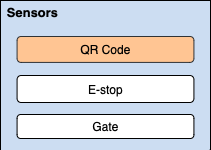
\includegraphics[width=0.60\textwidth]{images/qr.png}
 \caption{QR code subsystem description diagram}
\end{figure}

\subsubsection{Assumptions}
The QR scanner will interface with the Raspberry Pi. It will transmit the location data obtained from the scanner and any commands from our PC to control the robot arm. If, for any reason, the QR scanner is unable to read the QR code, such as due to low lighting conditions, it will not transmit any digital data to the Raspberry Pi.

\subsubsection{Responsibilities}
The QR scanner, mounted on the robot arm, reads QR codes on boxes. Each QR code contains location information indicating where the box should be positioned. The QR scanner is connected to a Raspberry Pi to transmit the digital data.

\subsubsection{Subsystem Interfaces}
\begin {table}[H]
\caption {Subsystem interfaces} 
\begin{center}
    \begin{tabular}{ | p{1cm} | p{6cm} | p{3cm} | p{3cm} |}
    \hline
    ID & Description & Inputs & Outputs \\ \hline
    \#01 & read QR code and send the data & \pbox{3cm}{image} & \pbox{3cm}{digital data}  \\ \hline
    \end{tabular}
\end{center}
\end{table}

\subsection{E-Stop}
E-Stops serve as safety features, allowing users to halt the robot in the event of unexpected actions or when they desire. This sensor can stop the program, regardless of the current processing state.

\begin{figure}[h!]
	\centering
 	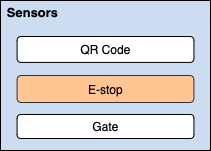
\includegraphics[width=0.60\textwidth]{images/stop.png}
 \caption{E-stop subsystem description diagram}
\end{figure}

\subsubsection{Assumptions}
When any of the E-stop buttons is pressed, the input value changes, and this value is then relayed to the controller to halt the system. E-stops can be pressed to immediately stop the robot in case of potential collisions, unexpected behavior, or excessive temperature increases.

\subsubsection{Responsibilities}
If users press any of the E-stops, the system stops by transmitting the changed input value to the controller.

\subsubsection{Subsystem Interfaces}

\begin {table}[H]
\caption {Subsystem interfaces} 
\begin{center}
    \begin{tabular}{ | p{1cm} | p{6cm} | p{3cm} | p{3cm} |}
    \hline
    ID & Description & Inputs & Outputs \\ \hline
    \#02 & E-stop signal & \pbox{3cm}{button status} & \pbox{3cm}{0 or not 0}  \\ \hline
    \end{tabular}
\end{center}
\end{table}

\subsection{Gate}
The gate sensor is a safety component that detects whether the gate is open or closed.

\begin{figure}[h!]
	\centering
 	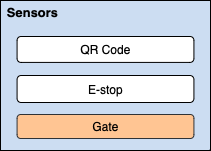
\includegraphics[width=0.60\textwidth]{images/gate.png}
 \caption{Gate subsystem description diagram}
\end{figure}

\subsubsection{Assumptions}
When the gate is open, the gate sensor sends a 'True' signal to the control, causing the robot to move slowly.

\subsubsection{Responsibilities}
Since the gate sensor detects value changes, it must transmit the changed value to the controller for a response.

\subsubsection{Subsystem Interfaces}
\begin {table}[H]
\caption {Subsystem interfaces} 
\begin{center}
    \begin{tabular}{ | p{1cm} | p{6cm} | p{3cm} | p{3cm} |}
    \hline
    ID & Description & Inputs & Outputs \\ \hline
    \#03 & Gate open or close & \pbox{3cm}{gate} & \pbox{3cm}{True or False}  \\ \hline
    \end{tabular}
\end{center}
\end{table}

